\documentclass[UTF8,12pt]{ctexart}
\usepackage{amsmath,amsthm,amsfonts,amssymb,bm,extarrows,graphicx,subfigure,booktabs,geometry,float}
\title{\hspace{50pt}\fontsize{68pt}{57pt}\bf 
$\ddot{\hat{\text{数}}}
{\overset{\Delta}{\ddot{\text{学}}}}
{\ddot{\tilde{\text{物}}}}
\ddot{\acute{\text{理}}}
\ddot{\vec{\text{\textcolor{white!76!black}{魔}}}}
$\\\hspace{52pt}
\kaishu\fontsize{45pt}{10pt} \textcolor{white!40!black}{及格手册}\hspace{10pt} \songti\bf$\fontsize{68pt}{30pt}{{\text{\textcolor{white!60!black}{法}}}}$\\\vspace*{0.7cm}\hspace{-20pt}
\fontsize{56pt}{10pt} \textcolor{white!68!black}{\heiti 复变函数}\textcolor{white!78!black}{\heiti 篇}}
\author{\zihao{-3}\tt \textcolor{white!0!black}{参宿四星云\quad 编}}
\date{\zihao{3}\kaishu\textcolor{white!40!black}{2023年1月13日}}
\geometry{papersize={210mm,297mm}}
\geometry{left=2.2cm,right=2.1cm,top=2.6cm,bottom=2.4cm}
\usepackage{fancyhdr}
\pagestyle{fancy}
\fancyhf{}
\fancyhead[L]{\S\thesection\ \leftmark}
\fancyhead[R]{\tt 参宿四星云}
\fancyhead[C]{\textcolor{white!60!black}{\heiti 复变函数魔法}}
\fancyfoot[C]{\thepage}
\usepackage{hyperref}
\usepackage{multicol}
\usepackage{vwcol}
\usepackage{lipsum,lmodern}
\usepackage{tcolorbox}
\usepackage{listings}
    \tcbuselibrary{skins, breakable, theorems}
%用法:$\stressbox{Formula}$
    \newcommand\stressbox{\tcboxmath[colframe=red,colback=yellow!50!white]}
    \newcommand\stressarea{\tcboxmath[colframe=yellow!50!white,colback=yellow!50!white]}
    \newcommand\stress{\tcboxmath[colframe=yellow!50!white,colback=yellow!50!white,left=0mm,right=0mm,top=0mm,bottom=0mm]}
    \tcbset{colback=white}

    \newenvironment{itemizer}{\begin{itemize}}{\end{itemize}}
    \tcolorboxenvironment{itemizer}{blanker,before skip=12pt,after skip=12pt,borderline west={3mm}{0pt}{red}}
    \newenvironment{itemizeg}{\begin{itemize}}{\end{itemize}}
    \tcolorboxenvironment{itemizeg}{blanker,before skip=12pt,after skip=12pt,borderline west={3mm}{0pt}{green!66!black}}
    \newenvironment{itemizeb}{\begin{itemize}}{\end{itemize}}
    \tcolorboxenvironment{itemizeb}{blanker,before skip=12pt,after skip=12pt,borderline west={3mm}{0pt}{blue}}
    
\usepackage{varwidth}

\usepackage{titlesec}
\usepackage{titletoc}
%标题
    \titleformat{\part}{\centering\Huge\bfseries}{第\,\chinese{part}\,部分}{1em}{}
    \titleformat{\section}{\centering\LARGE\bfseries}{\S\arabic{section}}{1em}{}
    \titleformat{\subsection}{\Large\bfseries}{{\arabic{section}.\arabic{subsection}}}{1em}{}
    \titleformat{\subsubsection}{\large\bfseries}{{\arabic{section}.\arabic{subsection}.\arabic{subsubsection}}}{1em}{}
    \titlespacing*{\part}{0pt}{-20pt}{20pt}
    \titlespacing*{\subsection}{-37.5pt}{0pt}{0pt}
    \titlespacing*{\subsubsection}{-35.5pt}{0pt}{0pt}
    %\titleformat{\subsection}{\bf}{\arabic{section}.\arabic{subsection}}{1em}{}
%目录
    \renewcommand{\contentsname}{\vspace*{-1.65cm}}
    \ctexset{section={name={\S}}}
    \titlecontents{part}[0em]{\vspace*{0.3cm}\heiti \Large}{\contentslabel{0em}}{}{\titlerule*[0.68pc]{}}
    \titlecontents{section}[2.2em]{\vspace*{0.3cm}\bf \large}{\contentslabel{2.0em}}{}{\titlerule*[0.68pc]{$\cdot$}\contentspage}


\newcommand{\I}{{\rm i}}
\newcommand{\pa}{\partial}
\newcommand{\tred}{\textcolor{red}}
\newcommand{\tblue}{\textcolor{blue}}

%用法:\begin{bbox}[options]{Title}
\newtcolorbox{bbox}[2][]{breakable,enhanced,skin=enhancedlast jigsaw,attach boxed title to top left={xshift=-4mm,yshift=-0.5mm},fonttitle=\bfseries\sffamily,varwidth boxed title=0.7\linewidth,colbacktitle=blue!45!white,colframe=blue!50!black,interior style={top color=white,bottom color=blue!6!white},boxed title style={empty,arc=0pt,outer arc=0pt,boxrule=0pt},underlay boxed title={\fill[blue!60!white] (title.north west) -- (title.north east)-- +(\tcboxedtitleheight-1mm,-\tcboxedtitleheight+1mm)-- ([xshift=4mm,yshift=0.5mm]frame.north east) -- +(0mm,-1mm)-- (title.south west) -- cycle;\fill[blue!45!white!35!black] ([yshift=-0.5mm]frame.north west)-- +(-0.4,0) -- +(0,-0.3) -- cycle;\fill[blue!45!white!35!black] ([yshift=-0.5mm]frame.north east)-- +(0,-0.3) -- +(0.4,0) -- cycle; },title={#2},#1}

\newtcolorbox{gbox}[2][]{breakable,enhanced,skin=enhancedlast jigsaw,attach boxed title to top left={xshift=-4mm,yshift=-0.5mm},fonttitle=\bfseries\sffamily,varwidth boxed title=0.7\linewidth,colbacktitle=green!65!white,colframe=green!60!black,interior style={top color=white,bottom color=green!6!white},boxed title style={empty,arc=0pt,outer arc=0pt,boxrule=0pt},underlay boxed title={\fill[green!76!black] (title.north west) -- (title.north east)-- +(\tcboxedtitleheight-1mm,-\tcboxedtitleheight+1mm)-- ([xshift=4mm,yshift=0.5mm]frame.north east) -- +(0mm,-1mm)-- (title.south west) -- cycle;\fill[green!45!white!45!black] ([yshift=-0.5mm]frame.north west)-- +(-0.4,0) -- +(0,-0.3) -- cycle;\fill[green!45!white!45!black] ([yshift=-0.5mm]frame.north east)-- +(0,-0.3) -- +(0.4,0) -- cycle; },title={#2},#1}

\newtcolorbox{wbox}[2][]{breakable,enhanced,skin=enhancedlast jigsaw,attach boxed title to top left={xshift=-4mm,yshift=-0.5mm},fonttitle=\bfseries\sffamily,varwidth boxed title=0.7\linewidth,colbacktitle=black!45!white,colframe=black!50!black,interior style={top color=white,bottom color=black!6!white},boxed title style={empty,arc=0pt,outer arc=0pt,boxrule=0pt},underlay boxed title={\fill[black!50!white] (title.north west) -- (title.north east)-- +(\tcboxedtitleheight-1mm,-\tcboxedtitleheight+1mm)-- ([xshift=4mm,yshift=0.5mm]frame.north east) -- +(0mm,-1mm)-- (title.south west) -- cycle;\fill[black!70!white] ([yshift=-0.5mm]frame.north west)-- +(-0.4,0) -- +(0,-0.3) -- cycle;\fill[black!70!white] ([yshift=-0.5mm]frame.north east)-- +(0,-0.3) -- +(0.4,0) -- cycle; },title={#2},#1}

\tikzset{coltria/.style={fill=red!15!white}}
\newtcolorbox{ebox}[1][]{empty,
breakable,height fixed for=first and middle,
leftrule=5mm,left=2mm,
frame style={fill,top color=red!10!yellow!80!black,bottom color=red!10!yellow!70!black,middle color=red!10!yellow!77!black},
colback=red!10!yellow!20!white,
% code for unbroken boxes:
frame code={\path[tcb fill frame] (frame.south west)--(frame.north west)
--([xshift=-5mm]frame.north east)--([yshift=-5mm]frame.north east)
--([yshift=5mm]frame.south east)--([xshift=-5mm]frame.south east)--cycle; },
interior code={\path[tcb fill interior] (interior.south west)--(interior.north west)
--([xshift=-4.8mm]interior.north east)--([yshift=-4.8mm]interior.north east)
--([yshift=4.8mm]interior.south east)--([xshift=-4.8mm]interior.south east)
--cycle; },
% code for the first part of a break sequence:
skin first is subskin of={emptyfirst}{%
frame code={\path[tcb fill frame] (frame.south west)--(frame.north west)
--([xshift=-5mm]frame.north east)--([yshift=-5mm]frame.north east)
--(frame.south east)--cycle;
\path[coltria] ([xshift=2.5mm,yshift=1mm]frame.south west) -- +(120:2mm)
-- +(60:2mm)-- cycle; },
interior code={\path[tcb fill interior] (interior.south west|-frame.south)
--(interior.north west)--([xshift=-4.8mm]interior.north east)
--([yshift=-4.8mm]interior.north east)--(interior.south east|-frame.south)
--cycle; },
},%
% code for the middle part of a break sequence:
skin middle is subskin of={emptymiddle}{%
frame code={\path[tcb fill frame] (frame.south west)--(frame.north west)
--(frame.north east)--(frame.south east)--cycle;
\path[coltria] ([xshift=2.5mm,yshift=-1mm]frame.north west) -- +(240:2mm)
-- +(300:2mm) -- cycle;
\path[coltria] ([xshift=2.5mm,yshift=1mm]frame.south west) -- +(120:2mm)
-- +(60:2mm) -- cycle;
},
interior code={\path[tcb fill interior] (interior.south west|-frame.south)
--(interior.north west|-frame.north)--(interior.north east|-frame.north)
--(interior.south east|-frame.south)--cycle; },
},
% code for the last part of a break sequence:
skin last is subskin of={emptylast}{%
frame code={\path[tcb fill frame] (frame.south west)--(frame.north west)
--(frame.north east)--([yshift=5mm]frame.south east)
--([xshift=-5mm]frame.south east)--cycle;
\path[coltria] ([xshift=2.5mm,yshift=-1mm]frame.north west) -- +(240:2mm)
-- +(300:2mm) -- cycle;
251
},
interior code={\path[tcb fill interior] (interior.south west)
--(interior.north west|-frame.north)--(interior.north east|-frame.north)
--([yshift=4.8mm]interior.south east)--([xshift=-4.8mm]interior.south east)
--cycle; },
},
#1}

\begin{document}
\everymath{\displaystyle}
\maketitle
\thispagestyle{empty}
\begin{tikzpicture}[even odd rule,overlay]
    \fill [opacity=.20](10,13) circle (200pt);
    \fill [opacity=.15](-10,2) circle (510pt) 
    (5,-10) circle (100pt) (0.2,9)circle(85pt);
    \fill [opacity=.25](9.2,-11.4) circle (60pt);
    \fill [opacity=.25](1.2,7)circle(21.4pt);
    \fill [opacity=.08](-1.2,-6)circle(46pt);
\end{tikzpicture}

\vspace*{3cm}
\begin{multicols*}{2}

\renewcommand\refname{参考文献}
\begin{thebibliography}{9}
    \bibitem[1]{1}黄发朋.数理方法讲义.
    \bibitem[2]{2}吴崇试,高春媛.数学物理方法.
    \bibitem[3]{3}吴崇试.数学物理方法习题指导.
    \bibitem[4]{4}黄志琦.数学物理方法简明导论.
    \bibitem[5]{5}林琼桂.数学物理方法.
\end{thebibliography}
\end{multicols*}

\newpage
\thispagestyle{empty}
\begin{center}
    \zihao{2}\bf 目录
\end{center}
%\begin{multicols*}{2}
    \tableofcontents   
%\end{multicols*}

\pagenumbering{arabic}
\newpage
\section{复变函数基础}

\begin{gbox}{可导性}
    若$\Delta z$以任意方式趋于0时,$\stress{\lim_{\Delta z\rightarrow 0}\frac{f(a+\Delta z)-f(a)}{\Delta z}\text{恒为一常数}}$,则称$f(z)$在$a$点可导。
\end{gbox}

\begin{gbox}{解析函数}
    若$f(z)$在区域$G$内处处可导,则称$f(z)$是$G$内的解析函数。
    \begin{itemizeg}
        \item[]解析函数无穷阶可导
    \end{itemizeg}
    \begin{wbox}{Cauchy-Riemann条件}
        \begin{equation}
            \begin{cases}
                \frac{\textcolor{red}{\partial u}}{\textcolor{red}{\partial x}}=\frac{\textcolor{blue}{\partial v}}{\textcolor{blue}{\partial y}}\vspace{8pt}\\
                \frac{\textcolor{red}{\partial u}}{\textcolor{blue}{\partial y}}=-\frac{\textcolor{blue}{\partial v}}{\textcolor{red}{\partial x}}\\
            \end{cases}\qquad
            \text{其中}f(z)=f(\tred{x}+\I\tblue{y})=\tred{u(x,y)}+\I \tblue{v(x,y)}.
        \end{equation}
    \end{wbox}
    \begin{equation}
        f(z)\text{可导(解析)}\Longleftrightarrow\begin{cases}
            \text{Cauchy-Riemann条件}\\
            \frac{\partial u}{\partial x},\frac{\partial u}{\partial y},\frac{\partial v}{\partial x},\frac{\partial v}{\partial y}\text{均连续}
        \end{cases}
    \end{equation}
    \tcbline
    \begin{equation}
        f(z)\text{可导(解析)}\Longrightarrow\begin{aligned}
            u(x,&y),\ v(x,y)\text{是{\bf 调和函数},即满足二维Laplace方程}\\
            &\begin{cases}\nabla^2 u=\left(\frac{\pa^2}{\pa x^2}+\frac{\pa^2}{\pa y^2}\right)u=0\vspace{5pt}\\
            \nabla^2 v=\left(\frac{\pa^2}{\pa x^2}+\frac{\pa^2}{\pa y^2}\right)v=0\end{cases}
        \end{aligned}
    \end{equation}
\end{gbox}


\newpage
\section{复变积分}
\subsection{Cauchy定理与Cauchy积分公式}

\begin{bbox}{Cauchy定理}
    若$f(z)$在闭曲线$C$包围的闭区域解析,那么(多连通区域亦可)
    \begin{equation}
        \stressbox{\oint_{C^+}f(z){\rm d}z=0}
    \end{equation}
    \tcbline
    有界单连通区域上的解析函数$f(z)$存在原函数$F(z)\equiv\int_{z_0}^zf(\zeta){\rm d}\zeta$,$F(z)$也称为$f(z)$的不定积分。
\end{bbox}

\begin{bbox}{Cauchy积分公式}
    $f(z)$在$\overline G$上是单值解析函数,分段光滑曲线$C$为$\overline G$的边界,则有
    \begin{equation}
        \stressbox{f(a)=\frac{1}{2\pi\I}\oint_{C^+}\frac{f(z)}{z-a}{\rm d}z}
    \end{equation}
    \paragraph*{推论}
    \begin{equation}
    \stressarea{f^{(n)}(a)=\frac{n!}{2\pi\I}\oint_{C^+}\frac{f(z)}{(z-a)^{n+1}}{\rm d}z}
    \end{equation}
\end{bbox}

\subsection{Jordan引理}
\setlength\columnsep{1.3cm}
\begin{multicols}{2}
\begin{wbox}{小圆弧引理}
    若$f(z)\in C\big(U^\circ(a)\big)$,并且在$\theta_1\leqslant\arg(z-a)\leqslant\theta_2$中,$(z-a)f(z)\rightrightarrows k\ (|z-a|\rightarrow 0)$,则有
    \begin{equation}
        \lim_{\rho\rightarrow 0}\int_{C_\rho}f(z){\rm d}z=\I k(\theta_2-\theta_1)
    \end{equation}
\end{wbox}

\begin{wbox}{大圆弧引理}
    若$f(z)\in C\big(U^\circ(\infty)\big)$,并且在$\theta_1\leqslant\arg(z-a)\leqslant\theta_2$中,$zf(z)\rightrightarrows K\ (z\rightarrow\infty)$,则有
    \begin{equation}
        \lim_{R\rightarrow\infty}\int_{C_R}f(z){\rm d}z=\I K(\theta_2-\theta_1).
    \end{equation}
\end{wbox}
\end{multicols}
\noindent 注:大、小圆弧引理中$K=0$或$k=0$非常常用。也有一些不满足一致收敛的情况使得复变积分收敛于0.

\begin{ebox}
    \tblue{\bf 计算菲涅尔积分$\int_{-\infty}^\infty \frac{\sin^2x}{x^2}{\rm d}x$}\

    \begin{equation}
        \frac{\sin^2x}{x^2}=\frac{1-\cos 2x}{2x^2}={\rm Re}\left\{\frac{1-e^{\I 2x}}{2x^2}\right\}
    \end{equation}
    设$g(x)=\frac{1-e^{\I 2x}}{2x^2}$,计算$g(x)$的围道积分,再用柯西定理。

    \begin{vwcol}[widths={0.54,0.35},rule=0pt]
        $L_2$大圆弧,设$x=Re^{\I\theta}$,则有

        $\begin{aligned}
            \lim_{R\rightarrow\infty}xg(x)
                &=\frac{1-e^{\I 2x}}{2x}=\frac{1-e^{-2R\sin\theta}e^{2\I R\cos\theta}}{2x} \\
            \because&\quad \left|e^{-2R\sin\theta}e^{2\I R\cos\theta}\right|\leqslant 1 \\
            \therefore&\quad xg(x)\rightrightarrows 0\ (R\rightarrow\infty)
        \end{aligned}$

        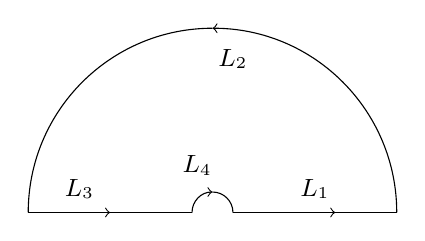
\begin{tikzpicture}[scale=1.3]
            \draw[->](0.2,0)--(1.2,0);\draw(1.2,0)--(1.8,0);
            \node[rotate=0] at (1.0,0.23){\small $L_1$};
            \draw[->](1.8,0)arc(0:90:1.8);\draw(0,1.8)arc(90:180:1.8);
            \node[rotate=0] at (0.2,1.5){\small $L_2$};
            \draw[->](-1.8,0)--(-1.0,0);\draw(-1.0,0)--(-0.2,0);
            \node[rotate=0] at (-1.3,0.23){\small $L_3$};
            \draw[->](-0.2,0)arc(180:90:0.2);\draw(0,0.2)arc(90:0:0.2);
            \node[rotate=0] at (-0.15,0.46){\small $L_4$};
        \end{tikzpicture}
    \end{vwcol}
    由大圆弧引理,$\int_{L_2}g(x){\rm d}x=0.$

    $L_4$小圆弧,有
    $$\lim_{x\rightarrow 0}xg(x)
    =\frac{1-e^{\I 2x}}{2x}=\frac{1-\left(1+\I 2x+o(x)\right)}{2x}=-\I+o(1)=-\I$$
    由小圆弧引理,$\int_{L_4}g(x){\rm d}x=-\pi.$

    积分路径不包围奇点,由柯西定理,
    $$\int_{-\infty}^\infty \frac{\sin^2x}{x^2}{\rm d}x=\int_{L_3+L_1}g(x){\rm d}x=-\int_{L_2+L_4}g(x){\rm d}x=\pi.$$
\end{ebox}


\newpage
\section{级数展开}

\subsection{Taylor展开}
函数$f(z)$在以$a$为圆心的圆$C$内解析,则对$\forall z\in C$,都可以展开为
\begin{equation}
    \stressbox{f(z)=\sum_{n=0}^\infty c_n(z-a)^n,\quad |z-a|<R}
\end{equation}
\paragraph*{系数求法}\
\begin{itemizeb}
    \item Cauchy积分公式:$\stress{c_n=\frac{f^{(n)}(a)}{n!}=\frac{1}{2\pi\I}\oint_{L^+}\frac{f(z)}{(z-a)^{n+1}}{\rm d}z,}$其中$L^+$为$C$内任一逆时针绕$a$一周的路径。
    \item 使用常用级数的线性组合、级数乘法、导数、积分、“待定系数法”(仅适用于有限个负幂项或正幂项的情况)。
\end{itemizeb}

\paragraph*{性质}\
\begin{itemizeg}
    \item 展开的形式与实变函数中相同
    \item Taylor展开、Laurent展开都具有唯一性
    \item $f(z)$的奇点完全决定其收敛半径
\end{itemizeg}

\subsection{Laurent展开}
函数$f(z)$在以$b$为圆心的环形区域$C:\ R_1<|z-b|<R_2$中单值解析,则对$\forall z\in C$,都可以展开为
\begin{equation}
    \stressbox{f(z)=\sum_{n=-\infty}^\infty c_n(z-b)^n,\quad R_1<|z-b|<R_2,}
\end{equation}
\begin{vwcol}[widths={0.6,0.4},rule=0pt]
其中$\stress{c_n=\frac{1}{2\pi\I}\oint_{L^+}\frac{f(z)}{(z-b)^{n+1}}{\rm d}z,}L^+$为$C$内任一逆时针绕$a$一周的路径。
\ \\ \ \\ \ \\ \ \\ \ \ \\ \ 
    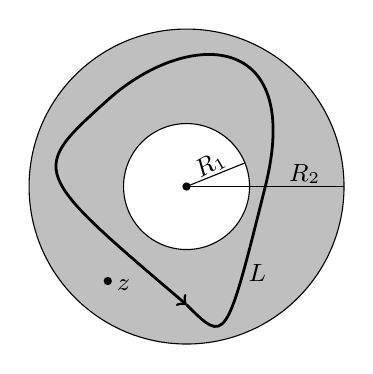
\begin{tikzpicture}[scale=1] 
        \fill[color=white!75!black](0,0)arc(0:360:2)(-1.2,0)arc(360:0:0.8);
        \draw[color=black](0,0)arc(0:360:2)(-1.2,0)arc(360:0:0.8);
        \draw(0,0)--(-2,0);
        \node at (-0.5,0.16){\small $R_2$};
        \draw(-2,0)--(-1.258,0.3);
        \node[rotate=30] at (-1.7,0.28){\small $R_1$};
        \fill (-2,0) circle (1.5pt);
        \fill (-3,-1.2) circle (1.5pt);
        \node at (-2.8,-1.25){\small $z$};
        \draw[line width=1pt,->] (-2,-1.5)..controls(-1.5,-2)..(-1,0)..controls(-0.5,2)and(-2,2)..(-3,1.1)..controls(-4,0.2)..(-2,-1.5);
        \node at (-1.1,-1.1){\small $L$};
    \end{tikzpicture}
\end{vwcol}

\begin{ebox}
    \textcolor{blue}{\bf 常用技巧: $|z|>1$时的几何级数展开}
    \begin{equation}
        \begin{aligned}
            \frac{1}{1-z}&=\frac{\frac{1}{z}}{\frac{1}{z}-1}\\
            &=-\frac{1}{z}\cdot \frac{1}{1-\frac{1}{z}}\\
            &=-\frac{1}{z}\cdot\sum_{k=0}^\infty \left(\frac{1}{z}\right)^k\\
            &=\sum_{k=-\infty}^{-1}(-1)z^k \qquad |z|>1
        \end{aligned}
    \end{equation}
\end{ebox}

\newpage
\section{留数定理}
\subsection{留数}

\begin{vwcol}[widths={0.65,0.35},rule=0pt]
    \indent 围绕解析函数$f(z)$的孤立的$\forall$奇点$b_k$作简单闭合曲线$\gamma_k$,则$f(z)$在$b$点的{\bf 留数}定义为
    \begin{equation}
        \stressbox{{\rm Res}f(b_k)\equiv \frac{1}{2\pi\I}\oint_{\gamma_k^+}f(z){\rm d}z=c_{-1}}
    \end{equation}
    即Laurent展开的$-1$次项系数。
    \ \\ \ 
    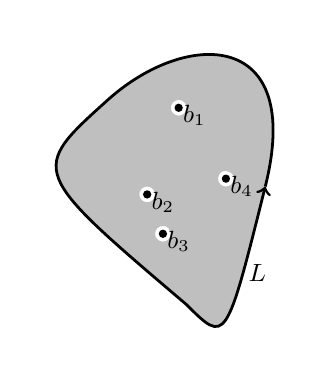
\begin{tikzpicture}[scale=1] 
        \fill[color=white!75!black] (-1,0)..controls(-0.5,2)and(-2,2)..(-3,1.1)..controls(-4,0.2)..(-2,-1.5)..controls(-1.5,-2)..(-1,0)
        --(-2,1)arc(360:0:0.1)
        --(-2.4,-0.1)arc(360:0:0.1)
        --(-2.2,-0.6)arc(360:0:0.1)
        |-(-1.5,0.2)arc(90:-270:0.1);
        \draw[line width=1pt,->] (-1,0)..controls(-0.5,2)and(-2,2)..(-3,1.1)..controls(-4,0.2)..(-2,-1.5)..controls(-1.5,-2)..(-1,0);
        \node at (-1.1,-1.1){\small$L$};
        \node at (-1.9,0.9){\small$b_1$}; \fill (-2.1,1) circle (1.5pt);
        \node at (-2.3,-0.2){\small$b_2$}; \fill (-2.5,-0.1) circle (1.5pt);
        \node at (-2.1,-0.7){\small$b_3$}; \fill (-2.3,-0.6) circle (1.5pt);
        \node at (-1.3,0){\small$b_4$};    \fill (-1.5,0.1) circle (1.5pt);   
    \end{tikzpicture}
\end{vwcol}        

\begin{gbox}{留数定理}
    若分段光滑简单闭合曲线$L$包围的区域中,除孤立奇点$b_1,\cdots,b_n$外$f(z)$单值解析,那么
    \begin{equation}
        \stressbox{\oint_{L^+}f(z){\rm d}z=2\pi\I\sum_{k=1}^n{\rm Res}f(b_k)}
    \end{equation}
\end{gbox}

\begin{wbox}{无穷远点的留数}
    若$\infty$不是非孤立奇点,那么可以定义
    \begin{equation}
        \stress{{\rm Res\ }f(\infty)=\frac{1}{2\pi\I}\oint_{C^-}f(z){\rm d}z}
    \end{equation}
    {\bf 留数和定理}
    \begin{equation}
        \sum_k{\rm Res\ }f(z_k)+{\rm Res\ }f(\infty)=0 
    \end{equation}
\tcbline
    若$\frac{-1}{t^2}f\left(\frac{1}{t}\right)$在$t=0$点邻域内展开为$\sum_{k=-\infty}^\infty a_kz^k$,则
    \begin{equation}
        \stress{{\rm Res\ }f(\infty)=a_{-1}}
    \end{equation}
\end{wbox}

\newpage
\subsection{留数的求法}
\subsubsection{直接展开法}
适用于较简单的分式、基本函数的线性组合等。可能需要对含无穷项的展开式使用几何级数展开等。
\begin{ebox}
    \begin{equation}\begin{aligned}
        \frac{1}{\sin z}&=\frac{1}{z-\frac{z^3}{3!}+o(z^4)}=\frac{1}{z}\frac{1}{1-\left(\frac{z^2}{3!}+o(z^3)\right)}\\
        &=\frac{1}{z}\left(1+\left(\frac{z^2}{3!+o(z^3)}\right)+\left(\frac{z^2}{3!+o(z^3)}\right)+\cdots\right)\\
        &=\frac{1}{z}+\frac{z}{3}+o(z^2)
    \end{aligned}\end{equation}
\end{ebox}

\subsubsection{待定系数法}
由于有“有限负幂项或有限正幂项”的限制,一般用来求有限阶极点的留数。
\begin{ebox}
    \textcolor{blue}
    {\bf 例:求$\frac{e^z}{\sin^2z}$在$z=0$点的留数\vspace{1em}\\}
    已知
    \begin{equation}
        \sin^2z=z^2-\frac{1}{3}z^4+o(z^5),\ e^z=1+x+o(x),
    \end{equation}
    初步判断$z=0$为2阶极点,设
    \begin{equation}
        \frac{e^z}{\sin^2z}=c_{-2}\frac{1}{z^2}+c_{-1}\frac{1}{z}+c_0+c_1z+o(z)
    \end{equation}
    则有
    \begin{equation}\left(c_{-2}\frac{1}{z^2}+c_{-1}\frac{1}{z}+c_0+c_1z+o(z)\right)\left(z^2-\frac{1}{3}z^4+o(z^5)\right)=1+z+o(z)
    \end{equation}
    对比$z$项系数,得到$c_{-1}=1.$
\end{ebox}

\subsubsection{画小圈圈法}
作$f(z)$的某单值解析域$G$内的简单闭合曲线$\gamma$,使$\gamma$只围绕奇点$b$,则
\begin{equation}
    \stress{{\rm Res}f(b)=\frac{1}{2\pi\I}\oint_{\gamma^+} f(z){\rm d}z}
\end{equation}

\subsubsection{大圆量级法}
若$f(z)=\frac{P(z)}{Q(z)}$且$P(z)$与$Q(z)$展开后的最高次项分别为$a_{n-1}z^{n-1}$与$b_nz^n$,且展开式在全复平面(或给定大小的圆之外)收敛,则$f(z)$在所有孤立奇点的留数之和为:
\begin{equation}
    \stress{\sum{\rm Res\ }z_k=\frac{a_{n-1}}{b_n}}
\end{equation}

(求除无穷原点外的所有奇点的留数和亦可使用“留数和定理”)

\subsubsection{升幂极限法}
若$z=b$是$f(z)$的$m$阶极点,即$f(z)=\sum_{k=-m}^\infty c_k(z-b)^k$.
\begin{itemizeb}
    \item 当$m=1,$\begin{equation}
        \stress{{\rm Res}f(b)=\lim_{z\rightarrow b}(z-b)f(z)}
    \end{equation}
    \item 当$m>1,\quad (z-b)^mf(z)=\sum_{k=-m}^\infty c_{k}(z-b)^{k-m}$只有正项级数和常数项,对其求$m-1$次导数后,常数项变为$c_{-1}(m-1)!$.        
\end{itemizeb}

\begin{ebox}
    \textcolor{blue}{\bf 例:求$\frac{1}{(e^z-1)^2}$在$z=0$点的留数\vspace{1em}\\}
    初步判断$z=0$为2阶极点。
    \begin{equation}
        z^2f(z)=\frac{z^2}{(e^z-1)^2}=c_{-2}+zc_{-1}+z^2c_0+\cdots
    \end{equation} 
    \begin{equation}
        \begin{aligned}
            \left(z^2f(z)\right)'&=\frac{2z(e^z-1)^2-z^2(e^z-1)\cdot 2e^z}{(e^z-1)^4}\\
            &=\frac{2z}{(e^z-1)^3}(e^z-1-ze^z)\\&=c_{-1}+2zc_0+3z^2c_1+\cdots
        \end{aligned}
    \end{equation}
    \begin{equation}
        \begin{aligned}
            \text{则}\lim_{z\rightarrow 0}\left(z^2f(z)\right)'&=2\cdot \frac{e^z-1-ze^z}{(e^z-1)^2}\\
            &=2\cdot \frac{z+\frac{1}{2}z^2+o(z^2)-z-z^2+o(z^2)}{(z+o(z))^2}\\
            &=2\cdot \frac{-\frac{1}{2}z^2+o(z^2)}{z^2+o(z^2)}\\
            &=-1
        \end{aligned}
    \end{equation}
\end{ebox}

\subsubsection{洛必达法}
若$z=b$是$f(z)$的一阶极点,且$f(z)$可写为$\frac{P(z)}{Q(z)}$,则
\begin{equation}
    \stress{{\rm Res}f(b)=\frac{P(b)}{Q'(b)}}
\end{equation}
 
\subsection{鞍点近似法}
鞍点近似法(又称拉普拉斯方法、最速下降法)在此处仅作最简单介绍。
用于近似计算形如
\begin{equation}
    I(M)=\int_Lg(z)e^{Mf(z)}{\rm d}z
\end{equation}
的积分,且满足$M$很大,$g(z)$(在$z_0$点)变化缓慢,积分路径经过解析函数$f(z)$的{\bf 实部的鞍点\ }$z_0$且基本沿着最速下降线,积分的主要贡献来自$z_0$的邻域。近似公式为:
\begin{equation}
    I(M)=g(z_0) e^{Mf(z_0)}\sqrt{\frac{2\pi}{M|f''(z_0)|}}
\end{equation}

\begin{vwcol}[widths={0.62,0.4},rule=0pt]
    证明如下:\vspace*{-5cm}
    $$\hspace*{-0.3cm}\begin{aligned}
        I(M)&=\int_Lg(z)e^{Mf(z)}{\rm d}z\\
        \text{(鞍点处泰勒展开)}&\approx\int_L{\rm d}zg(z)e^{M\left[f(z_0)+\frac{(z-z_0)^2}{2}f''(z_0)\right]}\\
        &= e^{Mf(z_0)}\int_L{\rm d}zg(z)e^{M\frac{(z-z_0)^2}{2}f''(z_0)}\\
        \text{(主要贡献为$z_0$的邻域)}&\approx e^{Mf(z_0)}\int_{z_0-\epsilon}^{z_0+\epsilon}{\rm d}zg(z)e^{-M\frac{(z-z_0)^2}{2}\big|f''(z_0)\big|}\\
        \text{(高斯积分)}&\approx g(z_0) e^{Mf(z_0)}\sqrt{\frac{2\pi}{M|f''(z_0)|}}
    \end{aligned}$$

    \begin{tikzpicture}[scale=2.6]
        \fill[color=white!80!black] (-1,-1)--(-1,1)--(1,1)--(1,-1);
        \fill[color=white!70!black] (-1,-0.7) .. controls (-0.6,-0.6) and (-0.3,-0.32) .. (-0.03,0) .. controls (-0.25,0.75) .. (-0.6,1)--(-1,1);
        \node[rotate=28] at (-0.6,0.1){\small "divergent"};
        \fill[color=white!90!black] (-1,-0.7) .. controls (-0.6,-0.6) and (-0.3,-0.32) .. (-0.01,-0.05) .. controls (0.1,-0.3) .. (0.5,-1)--(-1,-1);
        \node[rotate=28] at (0.13,-0.8){\small $\approx 0$};
        \fill[color=white!70!black] (1,0.82) .. controls (0.3,0.32) .. (0.03,0) .. controls (0.1,-0.3) .. (0.5,-1)--(1,-1);
        \node[rotate=28] at (0.68,-0.08){\small "divergent"};
        \fill[color=white!90!black] (1,0.82) .. controls (0.3,0.32) .. (0.01,0.05) .. controls (-0.25,0.75) .. (-0.6,1)--(1,1);
        \node[rotate=28] at (0.5,0.75){\small $\approx 0$};
        \node at (-0.6,0.9){$e^{Mf(z)}$示意};
        \draw[dotted](-0.6,-1) .. controls (-0.2,-0.8)and(-0.1,-0.5) .. (0,0) .. controls (0.1,0.5) .. (0.04,1);
        \node[rotate=35,color=white!45!black] at (-0.54,-0.83){\small Gaussian};
        \draw[->](0,-0.6)..controls(0.13,-0.5)..(0.1,-0.4);
        \draw[->](0.1,-0.4) .. controls (0,-0.3)and(-0.02,-0.1) .. (0,0) .. controls (0.03,0.15) .. (0.2,0.5);
        \draw(0.2,0.5)--(0.25,0.6);
        \node[rotate=0] at (0.2,0.35){\small $L$};
    \end{tikzpicture}
\end{vwcol}

\newpage













\titleformat{\section}{\LARGE\bfseries}{}{1em}{}
\titleformat{\subsection}{\Large\bfseries}{{\Alph{subsection}.}}{1em}{}
\titleformat{\subsubsection}{\large\bfseries}{{\arabic{subsection}.\arabic{subsubsection}}}{1em}{}
\titlespacing*{\part}{0pt}{-20pt}{20pt}
\titlespacing*{\section}{-20pt}{0pt}{0pt}
\titlespacing*{\subsection}{0pt}{0pt}{0pt}
\titlespacing*{\subsubsection}{0pt}{0pt}{0pt}

\fancyhead[L]{附录}
\fancyhead[R]{\tt 参宿四星云}
\fancyfoot[C]{\thepage}
\renewcommand\thesection{\Alph{subsection}}
\renewcommand\thesubsection{\Alph{subsection}}

\ctexset{section={name={}},subsection={name={}}}
\titlecontents{section}[0.2em]{\vspace*{0.3cm}\bf \large}{\contentslabel{2.0em}}{}{\titlerule*[0.68pc]{$\cdot$}\contentspage}




\section{附录}

\subsection{多值函数}
\setlength\columnsep{1.3cm}
\begin{multicols}{2}
    \begin{gbox}{多值函数(例)}
        \begin{subequations}
            \begin{align}
                \sqrt{z-a}&=\begin{cases}
                    \sqrt{r}e^{\I\theta}\\
                    -\sqrt{r}e^{\I\theta}
                \end{cases}\\
                \ln z&=\ln|z|+\I\arg z\\
                &\!\!\!\!\!\!\!\arcsin,\arccos,\arctan,z^\alpha,\cdots \notag
            \end{align}
        \end{subequations}
    \end{gbox}
    \begin{wbox}{宗量}
        宗量为引起多值性的含自变量的表达式,不完全等同于自变量。如根号下的表达式、ln()内的表达式。
    \end{wbox}
    \begin{gbox}{支点}
        对于$f(z)$的定义域$C$,若存在$z_0\in C$,当自变量$z$连续地绕$z_0$转一圈回到原来的位置时,$f(z)$的值不还原,则称$z_0$为$f(z)$的支点(branch point,又称枝点、分支点等)。
    \end{gbox}
    \begin{gbox}{Riemann面}
        若宗量辐角变化$n$个周期后$f(z)$的值才还原,则可认为宗量在$n$叶Riemann面上。一些情况下,Riemann面上的每个点通过多值函数$f$可与复平面上的点一一对应。其中,$\sqrt{z-a}$的Riemann面是二叶的,$\ln z$的Riemann面是无穷叶的。
    \end{gbox}
    \begin{gbox}{单值分支}
        将Riemann面沿连接两个支点的简单曲线割开,就得到若干个几乎完整的复平面,每个复平面就是一个单值分支,可以通过定义的方式,使得$f(z)$在每个单值分支上都是单值函数。
    \end{gbox}
\end{multicols}

\newpage
\subsection{$\Gamma$函数}

\begin{gbox}[interior style={top color=yellow!50!white,bottom color=yellow!50!white},watermark color=black,watermark text={$\Gamma(z)\equiv\int_0^\infty e^{-t}t^{z-1}{\rm d}t,\quad {\rm Re\ }z>0$}]{$\Gamma$函数的定义}
    \ \\ \begin{equation}\quad
    \end{equation}\ \ 
\end{gbox}

\begin{gbox}[interior style={top color=yellow!50!white,bottom color=yellow!50!white},watermark color=black,watermark text={${\rm B}(p,q)\equiv\int_0^1 t^{p-1}(1-t)^{q-1}{\rm d}t,\quad {\rm Re\ }p,{\rm Re\ }q>0$}]{$\rm B$函数的定义}
    \begin{equation}\quad
    \end{equation}\ \ 
\end{gbox}

\begin{itemizeg}\item[]\textcolor{green!60!black}{\bf 基本性质}
    \begin{subequations}\begin{align}
        \text{收敛域:}\mathbb{C}\setminus\{0,-1,-2,\cdots\}\\
        \Gamma(z+1)&=z\cdot\Gamma(z),\quad \Gamma(n+1)=n!\\
        \Gamma(z)\cdot\Gamma(1-z)={\rm B}(z,1-z)&=\frac{\pi}{\sin (\pi z)}\\
        \Gamma(1)=\Gamma(2)&=1\\
        \Gamma\left(\frac{1}{2}\right)&=\sqrt{\pi}\\
        {\rm Res\ }\Gamma(-n)&=\frac{(-1)^n}{n!},\quad n=0,1,2,\cdots\\
        {\rm B}(p,q)={\rm B}(q,p)&=\frac{\Gamma(p)\Gamma(q)}{\Gamma(p+q)}
    \end{align}\end{subequations}
\end{itemizeg}        

\begin{bbox}{Stirling公式}
    当$x\gg 1,\Gamma$函数的近似公式为
    \begin{subequations}\begin{align}
        \Gamma(x+1)=x!&\approx\sqrt{2\pi x}\left(\frac{x}{e}\right)^x\\
        \ln(n!)&\sim n\ln n-n
    \end{align}\end{subequations}
\end{bbox}

\begin{ebox}
    不难证明:
    \begin{subequations}
        \begin{align}
            \int_0^\infty e^{t^n}{\rm d}t&=\frac{1}{n}\Gamma\left(\frac{1}{n}\right)\\
            \int_0^\infty e^{\pm\I t^n}{\rm d}t&=\frac{1}{n}\Gamma\left(\frac{1}{n}\right)e^{\mp\frac{\I\pi}{2n}}
        \end{align}
    \end{subequations}
\end{ebox}

\begin{ebox}
    \textcolor{blue}{\bf 用$\Gamma$函数推导$n$维球体积的$R^n$项系数\\}
    设$n$维球:$x_1+x_2+\cdots+x_n\leqslant R^2$\\
    且$V_n=C_nR^n$,其中$C_n$是只与$n$有关的数,\\
    对上式微分,得到
    \begin{equation}
        {\rm d}V_n=C_n{\rm d}R^n=C_n n R^{n-1}{\rm d}R
    \end{equation}
    另外,有(高斯积分、$\Gamma$函数的重要性质)
    \begin{equation}
        \Gamma\left(\frac{1}{2}\right)=\int_0^\infty \frac{e^{-t}}{\sqrt{t}}{\rm d}t \xlongequal[{\rm d}t=2x{\rm d}x]{t=x^2} \int_0^\infty e^{-x^2}\frac{2x{\rm d}x}{x}=2\int_0^\infty e^{-x^2}{\rm d}x=\int_{-\infty}^\infty e^{-x^2}{\rm d}x=\sqrt{\pi}
    \end{equation}
    所以\begin{equation}
        \begin{aligned}
            \left(\sqrt{\pi}\right)^n&=\left(\int_{-\infty}^\infty e^{-x^2}{\rm d}x\right)^n\\
            &=\int\cdots\int_{-\infty}^\infty e^{-(x_1^2+\cdots+x_n^2)}{\rm d}x_1\cdots{\rm d}x_n\\
            &=\int e^{-R^2}{\rm d}V_n\\
            &=C_n n\int_0^\infty e^{-R^2}R^{n-1}{\rm d}R\\ 
            &\!\!\!\!\!\!\!\!\!\!\!\!\!\!\!\!\!\!\!\!\!\! 
            \xlongequal[{\rm d}R=\frac{1}{2\sqrt{t}}{\rm d}t]{R=\sqrt{t}}
            C_n \frac{n}{2}\int_0^\infty e^{-t}1t^{\frac{n}{2}-1}{\rm d}t
            \quad=C_n \frac{n}{2}\Gamma\left(\frac{n}{2}\right)\\ 
        \end{aligned}
    \end{equation}
    \begin{equation}
        \quad\Longrightarrow\quad C_n=\frac{2\pi^{\frac{n}{2}}}{n\Gamma\left(\frac{n}{2}\right)}
    \end{equation}
\end{ebox}

\begin{ebox}
    \textcolor{blue}{\bf 用B函数证明Wallis公式的一个中间结果}
    \begin{equation}
        \text{Wallis公式:}\qquad\lim_{n\rightarrow\infty}\frac{(2n)!!}{(2n-1)!!}\frac{(2n)!!}{(2n+1)!!}=\frac{\pi}{2}
    \end{equation}
    \begin{equation}
        \begin{aligned}
            \int_0^{\frac{\pi}{2}}\sin^n\theta{\rm d}\theta
            &\xlongequal[{\rm d}\theta=\frac{{\rm d}t}{\sqrt{1-t^2}}]{t=\sin\theta}\int_0^1\frac{t^n}{\sqrt{1-t^2}}{\rm d}t
            \xlongequal[{\rm d}t=\frac{{\rm d}u}{2\sqrt{u}}]{u=t^2}
            \frac{1}{2}\int_0^1 u^{\frac{n-1}{2}}(1-u)^{-\frac{1}{2}}{\rm d}u\\
            &=\frac{1}{2}{\rm B}\left(\frac{n+1}{2},\frac{1}{2}\right)
            =\frac{\Gamma\left(\frac{n+1}{2}\right)\Gamma\left(\frac{1}{2}\right)}{2\Gamma\left(\frac{n}{2}+1\right)}\\
            &=\begin{cases}
                \frac{(n-1)!!}{n!!},&n=2k+1,\quad k\in\mathbb{Z}^+\vspace{1em}\\
                \frac{(n-1)!!}{n!!}\frac{\pi}{2},&n=2k,\qquad k\in\mathbb{Z}^+\\
            \end{cases}
    \end{aligned}
    \end{equation}
以下略。
\end{ebox}


\end{document}